\begin{solution}

The key insight is to write the plane polarized light as the superposition of 2 circularly polarized light waves of the same frequency. 
\begin{center}
    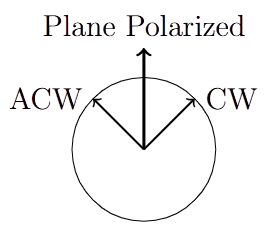
\includegraphics[width=0.25\textwidth]{solutions/figures/polarization-decomposition.png}
\end{center}
    
After passing through the solution, since they have different refractive indices $n_L$ and $n_R$, the phase difference between them is given by
$$\frac{\phi}{2\pi} = \frac{L}{\lambda_{\text{medium}}} = \frac{L}{\frac{\lambda}{n}} \implies \Delta \phi = \frac{2\pi}{\lambda}L\Delta n$$
    
However, note that this is the phase shift and not the rotation angle.

\begin{center}
    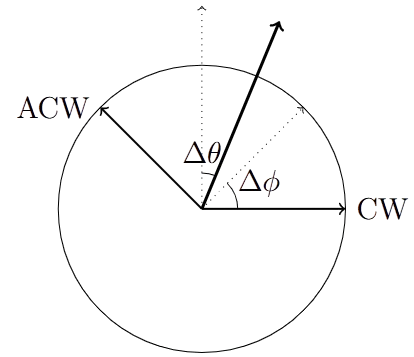
\includegraphics[width=0.3\textwidth]{solutions/figures/rotation-shift.png}
\end{center}
    
Hence $\Delta \theta = \frac{1}{2}\Delta \phi = \frac{\pi}{\lambda} L \Delta n$. Plugging the values in will give $\boxed{\Delta \theta = \frac{3\pi}{2} \approx 4.71\;\mathrm{rad}}$.

\end{solution}